\chapter{Design}
\label{sec:design}

% Ist das zentrale Kapitel der Arbeit. Hier werden das Ziel sowie die
% eigenen Ideen, Wertungen, Entwurfsentscheidungen vorgebracht. Es kann
% sich lohnen, verschiedene Möglichkeiten durchzuspielen und dann
% explizit zu begründen, warum man sich für eine bestimmte entschieden
% hat. Dieses Kapitel sollte - zumindest in Stichworten - schon bei den
% ersten Festlegungen eines Entwurfs skizziert werden.
% Es wird sich aber in einer normal verlaufenden
% Arbeit dauernd etwas daran ändern. Das Kapitel darf nicht zu
% detailliert werden, sonst langweilt sich der Leser. Es ist sehr
% wichtig, das richtige Abstraktionsniveau zu finden. Beim Verfassen
% sollte man auf die Wiederverwendbarkeit des Textes achten.

% Plant man eine Veröffentlichung aus der Arbeit zu machen, können von
% diesem Kapitel Teile genommen werden. Das Kapitel wird in der Regel
% wohl mindestens 8 Seiten haben, mehr als 20 können ein Hinweis darauf
% sein, daß das Abstraktionsniveau verfehlt wurde.

\ldots design \ldots

\todo{write design}
\begin{itemize}
    \item Current problem: as described in chapter 2.summary: no real protection against SCA
    \item Section first describes the environment
    \item Then describe the system as a whole
    \item then describe the tee kernel and requirements on it
\end{itemize}

\section{Environment}
\begin{itemize}
    \item PMC implementation Specific
    \item Intel and AMD use different address schemas
    \item AMD/Intel implements different events
    \item I focus on events compatible to processors derived from Skylake
    \item this means I'll support CPUs for this PoC of Skylake to Alderlake
    \item Want to use core local resources -> no HT at all
    \item I focus on the implementation of the TEE Software
    \item This means, I don't care much about the setup and that's left for
          future work
    \item in particular in this PoC I assume that software is not hostile until
          the TEE is running
    \item Want to research if I can employ a SC free software on a dedicated core
    \item I require the presence of a TPM
    \item TEE software runs isolated on core
    \item Performance counters monitor events regarding L3 cache usage
    \item If a request can't be served by L2 the TEE software terminates
\end{itemize}

\section{System description}
\begin{figure}
    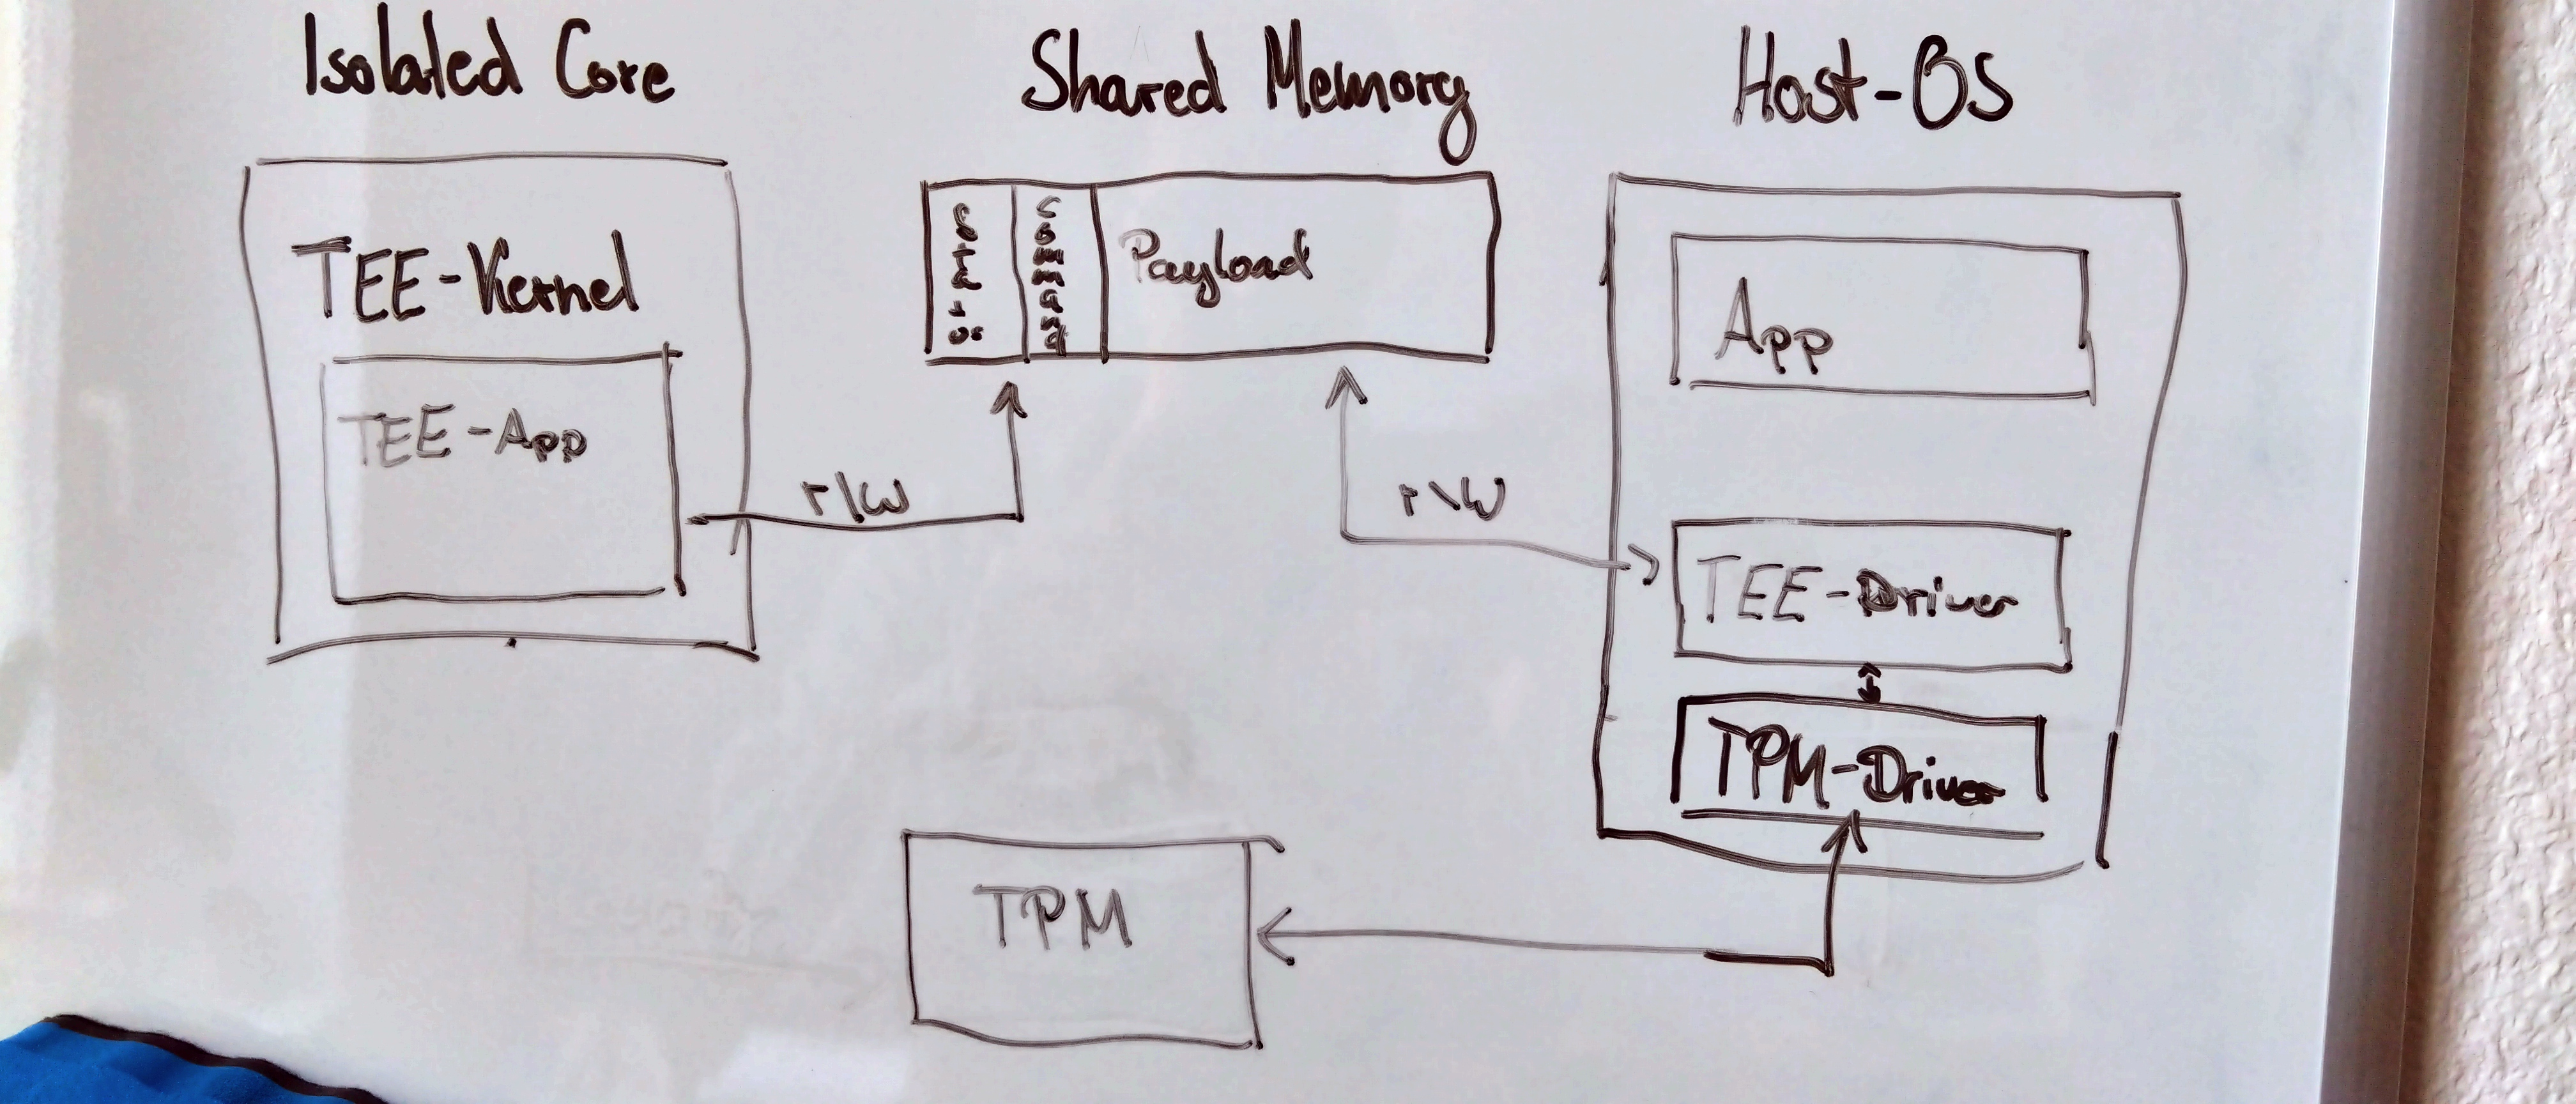
\includegraphics[width=.8\textwidth]{images/architecture.JPG}
\end{figure}
\begin{itemize}
    \item System consists of TEE Software, Host kernel on which user programs run,
          driver to communicate with TEE and TPM
    \item host and TEE communicate via driver
    \item this prototype only implements a subset of the standalone system
    \item therefore depends more on the host system
    \item generally: design constist of TEE kernel that offers services to other
          system components
    \item In most cases another OS runs on the same CPu package, owns the remaining parts of the system
    \item This is called the host system
    \item host is commodity general purpose operating system
    \item driver for host implements controlling routines for tee kernel
    \item tee kernel runs on dedicated core
    \item implements TEE services to allow shielded execution of code
    \item both host and tee utilize tpm to sign measurements or generate keys
    \item when system starts, firmware measures bootloader
    \item bootloader measures Teekernel and host OS, can check if TEE kernel is
          the expected one
    \item if so, loads tee kernel. This makes Firmware and bootloader part of the
          TCB
    \item Because implementation of TPm supporting bootloader is out of scope ->
          we use the host kernel to setup the TEE
    \item in other words: I trust the host OS to at least setup the TEE
          correctly in my PoC implementation
    \item I tell the host OS to not use specific resources
    \item If the host OS does not obey to these guidelines the TEE reacts in a fatal way
          that crashes the whole system
    \item The tee kernel and the Host OS communicate through shared memory
    \item - PMI can be delivered even if interrupts disabled
\end{itemize}

\section{TEE kernel}
\begin{itemize}
    \item TEE kernel must activate PMC as soon as possible
    \item Until PMC not enabled modifying attacks are possible
    \item Maps shared memory as uncacheable so communication does not influence PMCs
    \item Implements communication routines
    \item Manages resources of the isolated core
    \item 64 bit mode for later cryptographic
    \item Use secure boot to start
    \item offer communication interface to task
    \item runs task as communicated form host OS driver
    \item each task is a function
    \item tasks are allowed to use the shared memory channel for communication
    \item only defined tasks are supported
    \item at the end of an task TEE kernel reads PMCs and generates a report
          based on values \todo{Report generation not implemened yet}
    \item crashes system if forbidden access registers \todo{PMI not implemented yet}
    \item Important: does not protect leaks from happening but rather reacts to
          registered attacks
    \item Use TPM for RA \todo{Not implemened yet} of the
\end{itemize}

\section{Attacks}
\begin{itemize}
    \item Overall: Want to defend against an attack who can read memory
    \item Two subclasses: passive and active attacker
    \item Passive attacker reads memory and is able to retrieve secrets
    \item active attacker would be able to modify code/data in the TEE
    \item if active attack is possible this would pose a huge threat
    \item -> privilege escalation
    \item I can simulate such attacks by exposing memory intended for use by TEE
    \item Communicate physical address to host kernel
    \item For passive attacker read from this memory
    \item For active attacker also write from this memory
    \item After "attacker" finished read/write transfer control to TEE
    \item TEE reads/writes from memory which should be reflected by the right
          PMC events
\end{itemize}


\cleardoublepage

%%% Local Variables:
%%% TeX-master: "diplom"
%%% End:
